\subsection{Data Layer}
Der Data Accss Layer regelt den Zugriff auf die Orthofotos mit Bing Maps, sowie die Strassen und Fussgängerstreifen, welche mit Hilfe von OpenStreetMap Daten über die Mapquest API zur Verfügung gestellt werden. Die Daten werden von den entsprechenden Quellen heruntergeladen und für die Detektion in ein passendes Format aufbereitet.

\subsubsection{Mapquest}
\Gls{Mapquest} \cite{Mapquest} wird in diesem Projekt als Schnittstelle zu den OpenStreetMap Daten verwendet. Dazu bieten sich die Developer Accounts an, welche auf 15000 Abfragen pro Monat begrenzt sind, was unseren Abfrageumfang ausreichend abdeckt.
Folgende Daten benötigen wir von der API:
\begin{tabbing}[H]
    \hspace*{3cm}\=\hspace*{9cm}\= \kill
    Strassen: \> Der Suchalgorithmus folgen den Strassenverläufen, \\
     			\> was die Suche effizienter und einfacher werden lässt.\\
    Fussgängerstreifen: \> Schon erfasste Fussgängerstreifen werden mit den von uns  \\ \> Entdeckten verglichen und nur diejenigen, welche noch nicht in erfasst sind,\\ \> werden abgespeichert.
\end{tabbing}


\subsubsection{Application Key}
In der Tabelle ist der Application Key aufgeführt, der für das Projekt Crosswalk Deteciton eingesetzt wurde.
\\
\begin{table}[H]
	\begin{tabular}{ | p{6cm} | p{6cm}  | }
		\hline    
		Consumer Key &  YKqJ7JffQIBKyTgALLNXLVrDSaiQGtiI \\ \hline
		Consumer Secret & 3DO1eoLMxSqPH7Gk \\ \hline
		Key Issued & Fri, 09/25/2015 - 07:17 \\ \hline
		Key Expires & Never \\ \hline
	\end{tabular}
	\caption[MapQuest Application Key]{MapQuest Application Key}
\end{table}

\paragraph{Beispiel Abfragen}
Um den Entwicklern beim Erstellen der Abfragen zu unterstützen wird auf Webseite \cite{mapquestapi} ein Xapi Service Developer's Guide zur Verfügung gestellt.

\subparagraph{HTTP Request}
Bounding Box:  47.367,8.545,47.367,8.544 (Rapperswil)
\begin{itemize}
	\item \url{http://open.mapquestapi.com/xapi/api/0.6/node[highway=*][bbox=8.544,47.367,8.545,47.367]?key=YKqJ7JffQIBKyTgALLNXLVrDSaiQGtiI}
\end{itemize}

\newpage
\subparagraph{XML File Response}
Als Antwort auf den HTTP Request gibt es ein XML File, welches die Strassen in Form von Nodes beinhaltet.\\

\begin{python}
	<osm xmlns:xapi="http://jxapi.openstreetmap.org/">
	<node id="32860913" version="8"
	timestamp="2015-08-06T15:21:13Z" uid="6087"
	lat="47.2254172" lon="8.8175171">
	<tag k="highway" v="traffic_signals"/>
	</node>
	</osm>
\end{python}



\paragraph{Abfrage}
Um das Resultat einer Abfrage einzugrenzen, bietet die API diverse Parameter und Tags die angegeben werden können. Damit wir nicht zu viele API Requests haben, können wir eine \textbf{Bounding Box}, sowie den Tag \textbf{highway=*} verwendet werden. Damit ist nur noch eine Abfrage pro Bounding Box (ca. 2 auf 2 Kilometer) nötig. Im Code sieht dies folgendermassen aus:
\subparagraph{Python Request} Abfrage mit Verwendung der httplib2 Library. \\ 
\begin{python}
import httplib2

url =  'http://open.mapquestapi.com/xapi/api/0.6/node
		[highway=*][bbox=8.544,47.367,8.545,47.367]?
		key=YKqJ7JffQIBKyTgALLNXLVrDSaiQGtiI}'
resp, content = httplib2.Http().request(url)
\end{python}

Das Resultat der Abfrage ist im XML Format, Python bietet für die Verarbeitung von XML Daten die Library \textbf{ElementTree}.\\
In einem nächsten Schritt schränken wir das Resultat weiter ein. Denn nicht auf allen Strassen sind Fussgängerstreifen möglich. Für uns relevant sind:
\begin{itemize}
	\item road, trunk, primary, secondary, tertiary, unclassified, residential, service, trunk\_link, primary\_link, secondary\_link, tertiary\_link, pedestrian
\end{itemize}

Am Ende der Verarbeitung resultiert eine Liste aller relevanten Strassen und alle Fussgängerstreifen.
\newpage
\subsubsection{Bing Maps}
Die wichtigsten Daten für die Suche sind die Orthofotos, welche wir über Bing Maps beschaffen. Dabei hilft uns das Python Skript globalmaptiles.py, welches den Umgang mit dem QuadTree Format von Bing Maps und das Umrechnen der Koordinaten zu den entsprechenden Tiles stark vereinfacht. (Mehr dazu unter dem Abschnitt~\ref{subsec:tiles} auf der Seite~\pageref{subsec:tiles}). Das herunterladen der Bilder lässt sich parallelisieren, was die Performance enorm steigert. In Python kann dazu die Library \textbf{multiprocessing.dummy import Pool as ThreadPool} verwendet werden.

\paragraph{Beispiel Download} Im Nachfolgenden Code ist gezeigt, wie der parallele Download implementiert wird. \\
\begin{python}
from multiprocessing.dummy import Pool as ThreadPool
from PIL import Image
import urllib2
import StringIO

def start_download(urls):
     pool = ThreadPool(self.nb_threads)       
     images = pool.map(download_image, urls)
     pool.close()
     pool.join()
     return images

def download_image(url):
    request = urllib2.Request(url)
    response = urllib2.urlopen(request)
    content = response.read()
    image = Image.open(StringIO.StringIO(content))
    return image

\end{python}

Das Resultat des Downloads ist eine Liste mit den Orthofotos, welche im Anschluss von dem Suchalgorithmus weiter verwendet werden.
\newpage
\subsubsection{Tiles à la Google Maps}
\label{subsec:tiles}
\Gls{Maptiler} bietet auf ihrer Webseite \cite{Tiles} ein Python Script an, welches den Umgang mit Tiles stark vereinfacht. Unter anderem wird die Umrechnung von Meter zu Latitude/Longitude, Meter zu Pixel und Tiles zu QuadTree \cite{quadtree} (Bing Format für Tiles) zur Verfügung gestellt.\\

\begin{figure}[H]
	\centering
	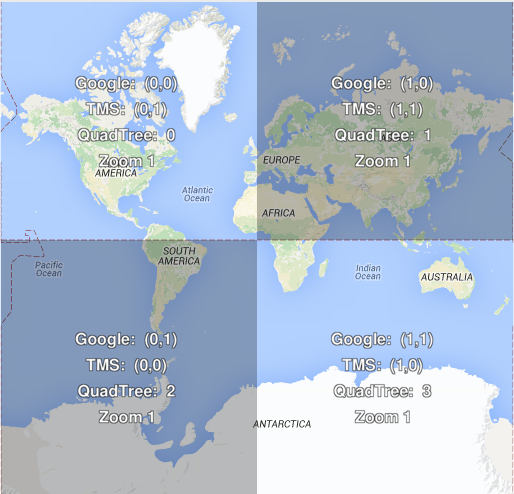
\includegraphics[width=150pt]{images/tiles_a_la_google.png}
	\caption[Tiles à la Google Maps]{Tiles à la Google Maps}
\end{figure}

\subsubsection{QuadKey}
Die \Gls{Quadkeys} von Bing Maps bauen sich wie auf der Abbildung ersichtlich auf. Jedes Zoomlevel führt dazu, dass der QuadKey um eine Stelle zu nimmt. Somit kann die Anzahl der Tiles für das ensprechende Zoomlevel mit dem Zoomlevel als Exponenten zur Basis 4 angegeben werden ($4^{Zoomlevel}$).  \\
\begin{figure}[H]
	\centering
	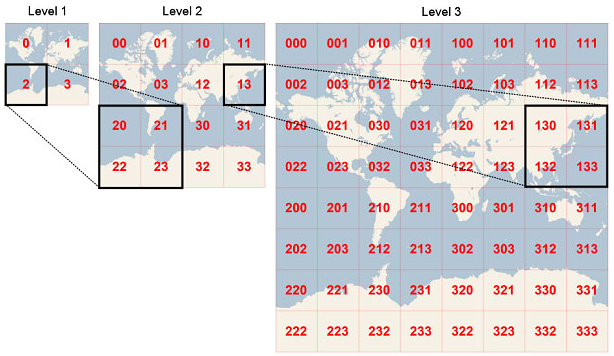
\includegraphics[width=300pt]{images/quadkey.png}
	\caption[QuadTree]{\Gls{QuadTree}}
\end{figure}
\newpage
\subsubsection{Beispiel Code}
Das folgende Beispiel zeigt die Umrechung vom WGS84 Koordinatensystem zu Meter, zu Tiles und schlussendlich zum Quadkey. (Auf dem Zoomlevel 19) \\
\begin{python}
	from src.data.globalmaptiles import GlobalMercator
	
	zoom = 19
	latitude = 47.0
	longitude = 8.0
	mercator = GlobalMercator()
	
	meter_x, meter_y = mercator.LatLonToMeters(latitude, longitude)
	tile_x, tile_y = self._mercator.MetersToTile(meter_x, meter_y, zoom)
	quadkey = mercator.QuadTree(tile_x, tile_y, zoom)
\end{python}



